\documentclass[aspectratio=169]{beamer}	 	

\usetheme{Goettingen}
\usecolortheme{default}
\usefonttheme{professionalfonts}			% para fontes matemáticas
% Enconte mais temas e cores em http://www.hartwork.org/beamer-theme-matrix/ 
% Veja também http://deic.uab.es/~iblanes/beamer_gallery/index.html

% Customizações de Cores: fg significa cor do texto e bg é cor do fundo

\definecolor{mypurple}{RGB}{75, 0, 130} % changed this
\definecolor{mypurple2}{RGB}{44, 0, 73} % changed this
\definecolor{mygray}{RGB}{250, 242, 250} % changed this
\definecolor{myblue}{RGB}{0, 0, 139} % changed this
\definecolor{baguete}{RGB}{255, 252, 255} % changed this

\setbeamercolor{normal text}{fg=black}
\setbeamercolor{alerted text}{fg=red}
\setbeamercolor{author}{fg=blue}
\setbeamercolor{institute}{fg=blue}
\setbeamercolor{date}{fg=myblue}
\setbeamercolor{frametitle}{fg=mypurple}
\setbeamercolor{framesubtitle}{fg=black}
\setbeamercolor{block title}{bg=mypurple2, fg=white}		%Cor do título
\setbeamercolor{block body}{bg=mygray, fg=darkgray}	%Cor do texto (bg= fundo; fg=texto)
\setbeamercolor{structure}{fg=mypurple}

\setbeamercolor{background canvas}{bg=baguete}

% informações do PDF
\makeatletter
\hypersetup{
     	%pagebackref=true,
		pdftitle={\@title}, 
		pdfauthor={\@author},
    	pdfsubject={Trabalho de Linguagem de programação em LaTeX},
	    pdfcreator={GLR, LSO, PS, THN},
		pdfkeywords={abnt}{latex}{abntex}{abntex2}{Linguagem de programação}, 
		colorlinks=true,       		% false: boxed links; true: colored links
    	linkcolor=black,          	% color of internal links
    	citecolor=blue,        		% color of links to bibliography
    	filecolor=magenta,      		% color of file links
		urlcolor=blue,
		bookmarksdepth=4
}
\makeatother

% ---
% PACOTES
% ---
\usepackage[alf]{abntex2cite}	% Citações padrão ABNT
\usepackage[brazil]{babel}		% Idioma do documento
\usepackage{color}			      % Controle das cores
\usepackage[T1]{fontenc}		  % Selecao de codigos de fonte.
\usepackage{graphicx}			    % Inclusão de gráficos
\usepackage[utf8]{inputenc}		% Codificacao do documento (conversão automática dos acentos)
\usepackage{txfonts}			    % Fontes virtuais
% ---

% --- Informações do documento ---
\title{Apresentando Haskell}
\author{Gustavo Lopes \and Lucas Santiago \and Pedro Souza \and Thiago Henriques }
\institute{Pontifícia Universidade Católica de Minas Gerais}
\date{26 de Março de 2021}
% ---

% ----------------- INÍCIO DO DOCUMENTO --------------------------------------
\begin{document}

    % ----------------- NOVO SLIDE --------------------------------
    \begin{frame}

    \begin{minipage}{1\linewidth}
      \centering
      \begin{tabular}{cc}
        \begin{tabular}{c}
          \includegraphics[width=3.0cm]{Haskell.png}
        \end{tabular}
      \end{tabular}
    \end{minipage}

    \titlepage

    \end{frame}

    %TABELA DE CONTEÚDO

    \AtBeginSection[]
    {
    \begin{frame}
      \frametitle{Conteúdo}
    \tableofcontents[currentsection]
    \end{frame}
    }

    % ----------------- NOVO SLIDE --------------------------------
    \section{Introdução}

    \begin{frame}{Introdução}
     
        \begin{columns}
          \column{0.3\textwidth}
          \textbf{Haskell} 
  
          \begin{itemize}
            \item O que é?
            \item Quando surgiu?
            \item Quem são os principais contribuidores?
            \item Qual o contexto que surgiu?
             
          \end{itemize}

          \column{0.6\textwidth}
  
          \begin{figure}  
          \includegraphics[width = 7.5 cm]{group_picture.png}
          \caption{\centering Membros e convidados IFIP Working Group 2.8, Disponível em \url{https://www.microsoft.com/en-us/research/wp-content/uploads/2016/07/history.pdf}}
          \end{figure}

        \end{columns}

    \end{frame}
    % ----------------- NOVA PARTE --------------------------------

    % ----------------- NOVO SLIDE --------------------------------
    \section{Histórico sobre a linguagem}
    \begin{frame}

      \frametitle{Histórico sobre a linguagem}
      \framesubtitle{com sua cronologia}

      \begin{columns}
        \column{0.3\textwidth}
        \textbf{Versões lançadas} 

        \begin{itemize}
          \item Haskell 1.0 
          \item Haskell 1.1
          \item Haskell 1.2
          \item Haskell 1.3
          \item Haskell 1.4 \pause
           
        \end{itemize}

        \column{0.6\textwidth}
        
        \begin{itemize}
          \item Haskell 98
          
          \begin{figure}  
            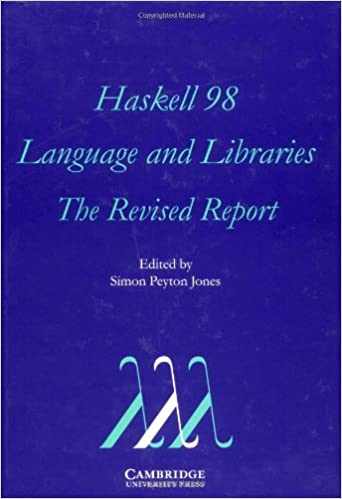
\includegraphics[scale=0.2]{book_haskell98.jpg}
            \caption{\centering Capa do livro do Haskell 98, Disponível em \url{https://images-na.ssl-images-amazon.com/images/I/41stT0WA1IL._SX340_BO1,204,203,200_.jpg}}
          \end{figure} 

        \end{itemize}

      \end{columns}

    \end{frame}
    % ----------------- NOVA PARTE --------------------------------
    \begin{frame}

      \frametitle{Histórico sobre a linguagem}
      \framesubtitle{com sua cronologia}

      \begin{columns}
        \column{0.3\textwidth}
        \textbf{Versões lançadas} 

        \begin{itemize}
          \item Haskell 2010 
          
          \begin{itemize}
            \item Módulos hierárquicos
            \item Regras de inferência
            \item Assuntos de sintaxe corrigidos
            \item Diretriz especificada     
          \end{itemize}

        \end{itemize}

        \column{0.6\textwidth}        

        \begin{figure}  
          \includegraphics[width = 7 cm]{report_haskell2010.png}
          \caption{\centering Relatório do Haskell 2010, Disponível em \url{https://www.haskell.org/definition/haskell2010.pdf}}
        \end{figure} 

      \end{columns}

    \end{frame}
    % ----------------- NOVA PARTE --------------------------------
    \begin{frame}
      
      \frametitle{Histórico sobre a linguagem}
      \framesubtitle{Status de Haskell atualmente}

      \begin{columns}
        \column{0.3\textwidth}
        \textbf{Haskell atualmente} 

        \begin{itemize}
          \item Programadores de Haskell cadastrados 
          \item Salário 
          \item Atualizações
        \end{itemize}

        \column{0.6\textwidth}

        \begin{figure}  
          \includegraphics[width = 8 cm]{haskell_org.png}
          \caption{\centering Homepage do site haskell.org, Disponível em \url{https://www.haskell.org/}}
        \end{figure} 

      \end{columns}

    \end{frame}
    % ----------------- NOVO SLIDE --------------------------------
    \section{Paradigma}

    \begin{frame}

      \frametitle{Paradigma}
      \framesubtitle{Definição}

      \begin{block}{O que é um 'Paradigma'?}
        Um Paradigma oferece e determina a visão que o programador possui sobre a estruturação
        e a execução do programa.
       \end{block} \pause 

       Exemplos:

       \begin{itemize}
         \item Orientada a Objeto (POO)
         \item Procedural
         \item Lógica de Programação
       \end{itemize}

    \end{frame}

    % ----------------- NOVO SLIDE --------------------------------
    \begin{frame}
      \frametitle{Paradigma}
      \framesubtitle{Imperativo \emph{Vs} Declarativo}

      \pause

      \begin{columns}
        \column{0.5\textwidth}
        \textbf{Imperativo} 

        \begin{itemize}
          \item Ações ou comandos que mudam o estado de um programa 
          \item "Faça isso, depois isso, depois aquilo..." \pause
        \end{itemize}

        \column{0.5\textwidth}

        \textbf{Declarativo} 
        \begin{itemize}
          \item Modelagem de um problema 
          \item Não há qualquer tipo de descrição de procedimentos
        \end{itemize}

      \end{columns}
    \end{frame}

    % ----------------- NOVO SLIDE --------------------------------
    \begin{frame}
      \frametitle{Paradigma Funcional}

      \begin{block}{Definição}
        Paradigma que descreve uma expressão matemática a ser avaliada,
        mapeando dos valores de entradas nos valores de retorno, por meio de funções.
      \end{block} \pause 

    \begin{figure}
      \includegraphics[scale=0.7]{ilustrativa.png}
      \caption{\centering ilustração da entrada de dados e saída de dados, Disponível em \url{http://www.inf.ufes.br/~vitorsouza/archive/2020/wp-content/uploads/teaching-lp-20132-seminario-haskell.pdf}}
    \end{figure}
       
    \end{frame}

    % ----------------- NOVO SLIDE --------------------------------
    \begin{frame}
      \frametitle{Paradigma Funcional}
      \framesubtitle{Características}

      \begin{block}{Dados imutáveis}
        Variáveis com tipagem forte, que são definidas e nunca mudam durante
        execução
      \end{block} \pause 

      \begin{block}{Funções puras}
        Recebem um parâmetro(input) e sempre vão retornar o mesmo, sem causar efeitos colaterais.
      \end{block} \pause 

      \begin{block}{Cálculo Lambda(Expressão Lambda)}
        Funões anônimas formadas por uma sequência de padrões
      \end{block} 
       
    \end{frame}

    % ----------------- NOVO SLIDE --------------------------------
    \begin{frame}
      \frametitle{Paradigma Funcional}
      \framesubtitle{Análise crítica}

      \pause

      \textbf{Vantagens} 
      \begin{itemize}
        \item Estruturas pequenas e de fácil compreensão \pause 
        \item Alto nível de abstração \pause 
      \end{itemize}

      \textbf{Desvantagens} 
      \begin{itemize}
        \item Difícil de se usar em contexto com muitas variáveis
        \\ Exemplo: Banco de Dados \pause  
        \item Ineficiência computacional 
      \end{itemize}
       
    \end{frame}

    %% Referencias dessa parte

    \nocite{haskellslides}
    \nocite{funcoespura}
    \nocite{funcoespura2}
    \nocite{haskellwikipedia}
    \nocite{paradigmas}

    %%

    % ----------------- NOVA PARTE --------------------------------

    % ----------------- NOVO SLIDE --------------------------------
    \section{Características mais marcantes}

    \begin{frame}
      \frametitle{Características mais marcantes}

      \begin{itemize}
        \item Como dito anteriormente, a linguagem só faz utilização de funções e funções dentro de funções. Por isso
        Haskell é descrito como puramente funcional. 
        \item Haskell possui uma sintaxe simples, elegante e concisa. Como resultado, programas em Haskell possuem 
        poucas linhas. 
        \item Além disso, a linguagem usa avaliação preguiçosa(Lazy evaluation), que é uma técnica para atrasar a computação 
        até um ponto em que o resultado da computação é considerado necessário.
        \item Tipagem estática: Verificação dos tipos usados em dados e variáveis para 
        garantir que sempre está sendo usado um tipo que é esperado em todas as situações. 
        \item Função de ordem superior: Função que tem como argumento uma outra função, ou que produz 
        uma função como resultado.
        \item Antes da execução de um programa, os compiladores e interpretadores realizam uma checagem forte de tipos
        de dados, verificação monomórfica e verificação polimórfica.
      \end{itemize}

    \end{frame}

    % ----------------- NOVA PARTE --------------------------------

    % ----------------- NOVO SLIDE --------------------------------
    \section{Relação com outras linguagens}

    \begin{frame}
      \frametitle{Relação com outras linguagens}
      \framesubtitle{Usando a suíte abnTeX2}

      \begin{itemize}
        \item Haskell vs Prolog
        \item Haskell vs Elixir
      \end{itemize}

    \end{frame}

    % ----------------- NOVA PARTE --------------------------------

    % ----------------- NOVO SLIDE --------------------------------
    \section{Exemplo(s) de programa(s)}

    \begin{frame}
      \frametitle{Exemplo(s) de programa(s)}

      \begin{figure}
        \includegraphics[width = 7 cm]{GHC.png}
        \caption{\centering HomePage do compilador GHC, Disponível em \url{https://www.haskell.org/ghc/}}
      \end{figure}

    \end{frame}

    % ----------------- NOVO SLIDE --------------------------------
    \section{Considerações finais}

    \begin{frame}
      \frametitle{Considerações finais}

      \begin{figure}
        \includegraphics[scale = 0.3]{questionamento.png}
        \caption{\centering Disponível em \url{https://www.focus.jor.br/wp-content/uploads/2018/01/Interroga\%C3\%A7\%C3\%A3o-e1516276871488.jpg}}
      \end{figure}


    \end{frame}
    % ----------------- NOVO SLIDE --------------------------------
    \section{Referências}

    % --- O comando \allowframebreaks ---
    % Se o conteúdo não se encaixa em um quadro, a opção allowframebreaks instrui 
    % beamer para quebrá-lo automaticamente entre dois ou mais quadros,
    % mantendo o frametitle do primeiro quadro (dado como argumento) e acrescentando 
    % um número romano ou algo parecido na continuação.

    \begin{frame}[allowframebreaks]{Referências}
      \bibliography{abntex2-modelo-references}
    \end{frame}

% ----------------- FIM DO DOCUMENTO -----------------------------------------
\end{document}